

% Language setting
% Replace `english' with e.g. `spanish' to change the document language

\documentclass[11pt]{article}
\usepackage[french]{babel}
\usepackage{wrapfig}
\usepackage{tikz}
\usepackage[a4paper,top=2cm,bottom=2cm,left=3cm,right=3cm,marginparwidth=1.75cm]{geometry}
\usepackage{amsmath}
\usepackage{graphicx}
\usepackage{varwidth}
\usepackage{algpseudocode}
\usepackage[colorlinks=true, allcolors=blue]{hyperref}
\usepackage[T1]{fontenc} 
\usepackage{xcolor}
\usepackage{minted}
\definecolor{bg}{HTML}{F8F8F8}






\title{ENSEIRB-MATMECA I1\\Rapport de projet d'algorithmique et de programmation n°2  \\
\begin{figure}[h]
\begin{tikzpicture}[scale=1.3]
\draw (0,0) -- (12,0);  
\end{tikzpicture}
\end{figure}
\vspace{1cm}
\textbf{\Huge Tower Defense}}
\vspace{1cm}

\author{ \\ Abderahim LAGRAOUI \\ Majid MEDGHALI  \\ Moussa ALLOUBANE\\ Mohammed BOUHAJA \\\\\\\textbf{Encadrant:} LOMBARDY Sylvain}
\date{}
\usepackage{fancyhdr}
\pagestyle{fancy}

\renewcommand{\headrulewidth}{1pt}
\fancyhead[]{} 
%\fancyhead[C]{\textbf{page \thepage}} 
%\fancyhead[L]{\leftmark}
%\fancyhead[R]{machin}
\renewcommand{\footrulewidth}{1pt}
\fancyfoot[C]{{\thepage/14}} 
\fancyfoot[L]{Projet de programmation N°2}
\fancyfoot[R]{Année 2022/2023}


\begin{document}

\maketitle
\begin{figure}[h]
    \centering
    
\includegraphics[height = 8cm , width = 14cm]{LOGO_EM.png}
\end{figure}
\newpage
\tableofcontents
    \newpage
    \section{Introduction}
        \subsection{Présentation générale du projet}
            Le jeu de défense de tours (ou Tower Defense en anglais) est un jeu stratégique où le joueur doit défendre un point ou une base en construisant des tours défensives sur un terrain de jeu. Comme l'illustre la figure~\ref{fig:tower defense}, les ennemis attaquent la base du joueur en suivant un chemin prédéfini, et le joueur doit utiliser des ressources pour placer les tours de manière stratégique afin de vaincre les vagues d'ennemis.
            Le projet en question vise à mettre en œuvre une version en TypeScript de ce jeu, en s'appuyant sur les connaissances acquises dans le cadre du cours de Programmation Fonctionnelle.
            \begin{figure}[h]
                \centering
                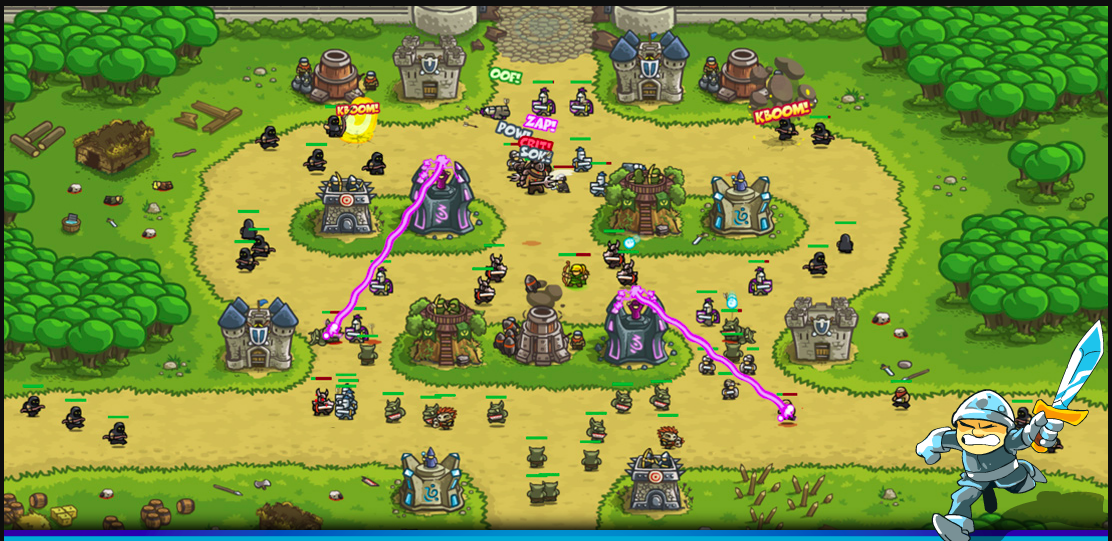
\includegraphics[height = 6cm, width = 10cm]{tower_defense_image.png}
                \caption{Tower Defense}
                \label{fig:tower defense}
            \end{figure}
        
        \subsection {Problématique}
             La problématique principale était de comprendre et de faire une abstraction du jeu en appliquant tous les aspects de la programmation fonctionnelle, de bien échanger les idées et les connaissances au sein du groupe et de savoir les acheminer pour résoudre les différentes difficultés aux niveaux de compilation, organisation du dépôt et synchronisation des travaux faits par chaque contributeur. 
             % De plus, l'exercice c'était de implémenter un code qui se base sur les structures de données et les fonctions prédéfinies dans la version de base.
        \subsection{Difficultés}
            Le projet en question présente plusieurs difficultés inhérentes à la conception du jeu à l'aide des principes de la programmation fonctionnelle plutôt que de la programmation impérative. La définition des types de base a particulièrement représenté un défi considérable, d'autant plus que l'implémentation initiale s'effectuait en JavaScript. De plus, il a été nécessaire de recourir à une approche impérative à certains moments et de procéder à la conversion vers une approche fonctionnelle ultérieurement.
        \subsection{Architecture du projet}
           Le projet en question est composé d'un ensemble de fichiers écrits en langage de programmation TypeScript. Afin de compiler le projet, l'outil Makefile est utilisé, comportant trois règles principales, à savoir $build$ pour compiler l'ensemble des fichiers, $run$ pour exécuter les fichiers générés en $js$, et $test$ pour compiler les fichiers de tests et mesurer leur couverture. Pour organiser les travaux, l'outil Git est employé, qui permet de travailler sur une version centrale tout en synchronisant les sources. En ce qui concerne la modularité, la figure~\ref{fig:diagramme} illustre le graphe de dépendances des fichiers, dont la plupart sont dépendants de $defineType.ts$, qui définit tous les types utilisés dans le projet. Il est à noter qu'une si une flèche arrive à un fichier, cela exprime la dépendance de ce fichier du fichier correspondant à la source de la flèche.
              \begin{figure}[h]
                \centering
                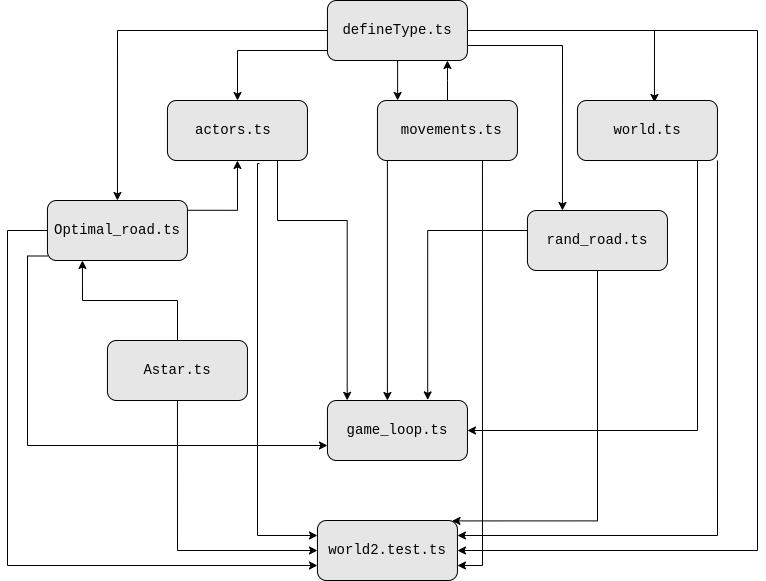
\includegraphics[height = 10cm, width = 15cm]{Diagramme sans nom.jpg}
                \caption{Graphes des dépendances}
                \label{fig:diagramme}
            \end{figure}
        \subsection{Organisation du projet}
       Les tâches de ce projet n'ont pas été préalablement définies, mais plutôt élaborées progressivement à travers des discussions sur les idées. Après s'être mis d'accord sur une abstraction du jeu, les membres de l'équipe ont commencé à mettre en œuvre ces idées en élaborant les types et les structures de données du monde, une responsabilité assumée par $Abderahim$ et $Majid$. $Mohammed$ s'est occupé de définir les fonctions liées aux attaques et au positionnement des tours sur la grille, tandis que $Moussa$ a cherché à valider son travail par des tests multiples. Par la suite, $Majid$ a pris en charge l'initialisation du monde, ainsi que la mise en place des fonctions de déplacement des monstres et de la boucle de jeu principale. $Moussa$ s'est ensuite chargé de la rédaction des fonctions de phase et du moteur du jeu, tandis qu'$Abderahim$ a implémenté et adapté l'algorithme A* pour le jeu. Enfin, $Mohammed$ a ajusté la gestion du flux entrant et sortant des monstres dans le monde. Concernant le rapport, chaque membre de l'équipe a écrit les sections du rapport liées aux tâches qu'il a assumé.
            
    \section{Définition du monde }
        \subsection{Tableau du jeu}
            Le monde du jeu est supposé une grille 2D rectangulaire de taille $width*height$, au sein de laquelle plusieurs types d'espèces interagissent les unes avec les autres. Les êtres présents sur la grille, tels que les routes, les sols, les monstres, les arbres, etc., sont appelés acteurs, chacun possédant des propriétés et des comportements distincts. D'une part, on parle des acteurs actifs tels que les monstres et les tours, et d'autre part, il y a les acteurs passifs tels que les arbres et le sol qui ne subissent pas de modifications d'état pendant le jeu.
        \subsection{Relations définies sur le monde}
            Compte tenu de la dynamique de mouvement propre à chaque acteur, il est indispensable de souligner les relations qu'il maintient avec ses voisins. Dans le modèle choisi, plusieurs possibilités de déplacements des acteurs ont été introduites, ce qui permet à chaque position de la grille de posséder jusqu'à huit voisins dans les huit directions cardinales et non-cardinales. Par ailleurs, chaque position peut être occupée par un seul acteur au maximum.
        \subsection{Acteurs du monde}
            Les acteurs représentent la première entité principale dans la grille. Ils sont définis comme un type de données doté d'un ensemble de propriétés les décrivant, tel que cela sera précisé ultérieurement dans la section~\ref{liste_acteurs}. Il est proposé d'avoir une implémentation unique qui rassemble tous les types d'acteurs, de telle sorte que tous les acteurs, par exemple, disposent d'une fonction de déplacement $Move$, même si cette fonctionnalité concerne uniquement les monstres. Le choix de cette implémentation repose sur la facilité de manipulation de ce type dans la suite du projet.
    \section{Construction du jeu}
    Suite à la discussion générale du sujet dans la section précédente, il est maintenant temps de procéder à une analyse plus détaillée de l'implémentation du jeu.
        \subsection{Définition des structures de données}
            La précision des types abstraits du projet, est une phase primordiale car elle permet de bien concrétiser les idées et de garder le lien entre les concepts abstraits du jeu et les idées algorithmiques permettant de les mettre en place.
            \subsubsection{Types principaux}
            Le premier type principal c'est $actor$, comme c'est illustré dans la figure~\ref{fig: type_actor } un acteur dispose d'une fonction de déplacement $Move$, d'un type $Type$ qui permet de distinguer les différents types d'acteurs, d'une couleur $Color$ utile pour son affichage dans la grille, d'un nombre de points de vie $HitPoints$ qui concerne uniquement les monstres et de deux champs $AttackRange$ et $Damage$ qui sont les propriétés des tours.
            % \begin{figure}[h]
            %     \centering
            %     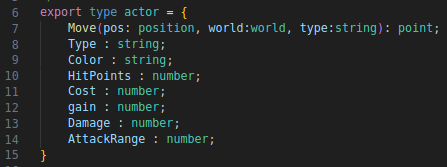
\includegraphics[height = 4.5cm, width = 12cm]{type_actor.png}
            %     \caption{Le type actor} 
            %     \label{fig: type_actor } 
            % \end{figure}

               \begin{figure}[h]
                \centering
                % 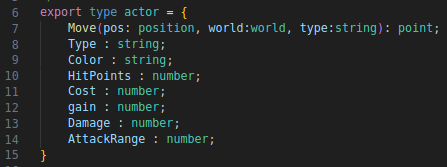
\includegraphics[height = 4.5cm, width = 12cm]{type_actor.png}
            \begin{minted}[bgcolor=bg, linenos=true, fontsize=\footnotesize]{typescript}
            export type actor = {
    Move(pos: position, world:world, type:string): point;
    Type : string;
    Color : string;
    HitPoints : number;
    Cost : number;
    gain : number;
    Damage : number;
    AttackRange : number;
}  \end{minted}
                \caption{Le type actor} 
                \label{fig: type_actor } 
            \end{figure}
            
            Le deuxième type, appelé type $world$, est illustré dans la figure~\ref{fig: type_world }. Ce type contient une matrice de type $position$ de taille $Width*Height$, ainsi qu'un tableau $Actors$ répertoriant les positions des monstres présents dans le monde. De même, un autre tableau nommé $Towers$ rassemble les positions des tours du monde, et enfin le score du joueur $Score$ est également inclus dans ce type.
            % \begin{figure}[h]
            %     \centering
            %     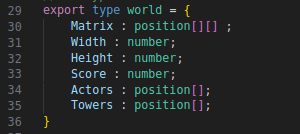
\includegraphics[height = 4cm, width = 10cm]{type_world.png}
            %     \caption{Le type world} 
            %     \label{fig: type_world } 
            % \end{figure}
            \begin{figure}[h]
            \centering
            \begin{minted}[bgcolor=bg, linenos=true, fontsize=\footnotesize]{typescript}
            export type world = {
                Matrix: position[][] ;
                Width: number;
                Height: number;
                Score: number;
                Actors: position[];
                Towers: position[];
            }
            \end{minted}
            \caption{Le type world} 
            \label{fig: type_world } 
            \end{figure}
            Deux autres types de base sont utilisés. Un point de la grille $point$ contient les deux coordonnées x et y comme le montre la figure~\ref{fig: type_point_position } et un type $position$ qui contient un point $Pos$ et un acteur $AnActor$ selon la même figure. Il convient de noter que dans ce contexte, une position est définie comme un point de la grille qui est occupé par un acteur.
            %  \begin{figure}[h]
            %     \begin{minipage}[c]{.45\linewidth}
            %         \centering
            %         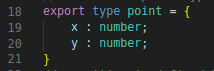
\includegraphics[height=2cm, width = 6cm]{type_point.png}
            %         \caption{Le type point}
            %         \label{fig: type_point}
            %     \end{minipage}
            %     \hfill%
            %     \begin{minipage}[c]{.45\linewidth}
            %           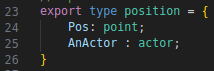
\includegraphics[height=2cm, width = 6cm]{type_position.png}
            %             \caption{Le type position} 
            %             \label{fig: type_position } 
            %     \end{minipage}
            % \end{figure}
\begin{figure}[h]
            \centering
            \begin{minted}[bgcolor=bg, linenos=true, fontsize=\footnotesize]{typescript}
            //this is the point type : a position x,y in the grid
export type point = {
    x : number;
    y : number;
}
//a position is defined by two coordinates and an actor occupying that position
export type position = {
    Pos: point;
    AnActor : actor;
}
            \end{minted}
            \caption{Les types point et position} 
            \label{fig: type_point_position } 
            \end{figure}
        
         \subsubsection{Liste des acteurs}\label{liste_acteurs}
            Les acteurs du monde ont des comportements variés, bien que leur implémentation soit uniforme. Chaque type d'acteur possède des propriétés particulières. Le modèle inclut deux types de monstres: $SimpleMonster$ et $BigMonster$. Le monstre simple effectue un déplacement basique vers une position voisine disponible, tandis que le grand monstre se déplace en suivant un chemin optimal tracé par l'algorithme $A*$, qui sera présenté dans la section~\ref{optimal chemin}. En outre, le grand monstre inflige davantage de dégâts que le monstre simple.
            
            Les structures de tours se différencient également. Deux types sont distingués: \textit{SimpleTower} et $MagicTower$. Les tours simples ont un champ de tir de 2 unités de surface et infligent des dégâts de 1 point, tandis que les tours magiques ont une puissance de tir avec une unité de plus. À noter que, sauf au début où le joueur dispose d'un certain nombre de tours gratuites, la construction de nouvelles tours est facturée à un coût spécifique qui sera déduit du score du joueur.
        \subsection{Généricité des mondes}
            L'implémentation du jeu présente un aspect de généricité important. Cet aspect se voit en deux points principaux, la génération aléatoire des chemins qui lient l'entrée et la sortie des monstres ainsi que le positionnement initial des tours et des arbres. 
            \subsubsection{Chemins aléatoires}
           Pour donner aux monstres la possibilité de gagner la partie, il faut tracer au moins un chemin entre la position d’entrée des monstres et une position finale qui représente l’objectif à atteindre. 
           
           Pour cela, on a choisit de créer des chemins aléatoires sur la grille de telle sorte d'assurer l'existence d'un tel chemin. Le choix retenu est l’algorithme de calcul en profondeur ou \textit{Depth-First Search} en anglais. Son principe est le suivant, on commence au début de chaque partie par fixer les deux positions initiale \textit{start} et finale \textit{end}. 
           
           Ensuite, on stocke le premier élément \textit{start}  dans un tableau des visiteurs. Ensuite, on applique l’algorithme \textit{DFS} qui teste si la case courante est égale à la position \textit{end}. Si oui on s'arrête et on retourne le tableau des visiteurs. Sinon, on détermine ses voisins et on les parcourt dans un ordre aléatoire en appliquant \textit{DFS} de manière récursive. À chaque appel, le tableau des visiteurs est mis à jour. 
           
           À la fin, on se retrouve avec un tableau des visiteurs qui contient un chemin qui relie les deux positions \textit{start} et \textit{end}. La figure~\ref{fig RandomRoad } donne un exemple d'une grille générée avec cet algorithme.
           \begin{figure}[h]
                \centering
                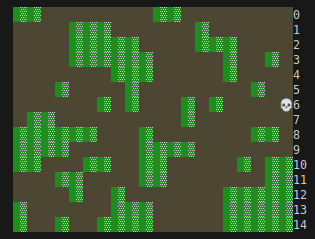
\includegraphics[height = 5cm, width = 8cm]{RandomRoad.png}
                \caption{Grille avec des chemins aléatoires} 
                \label{fig RandomRoad } 
            \end{figure}
            \subsubsection{Positionnement des tours}
            Les tours constituent le deuxième élément clé du monde et leur emplacement doit être choisi avec soin afin de permettre une résistance efficace aux monstres mais il doit aussi offrir la possibilité aux monstres d'accéder au monde. 
            
            À cet effet, l'approche suivante est employée : les positions de la grille sont examinées et celles qui possèdent au moins quatre positions voisines qui correspondent à des chemins sont regroupées. La moitié de ces positions est ensuite sélectionnée pour y placer les tours, ce qui garantit leur résistance face aux assauts des vagues de monstres. La figure~\ref{fig: positionnement } illustre à cette approche.

            \subsubsection{Positionnement des arbres}
            
            Pour ce qui est des arbres, le même principe est appliqué en utilisant l'autre moitié de la liste des positions sélectionnées pour les tours. Bien que les arbres ne soient pas des acteurs actifs aussi importants que les tours, leur emplacement doit être choisi avec soin pour conserver une apparence réaliste du jeu, en les disposant à proximité des chemins. La figure~\ref{fig: positionnement } illustre à cette approche, c'est une grille de jeu avant l'entrée des monstres. 

            \begin{figure}[h]
                \centering
                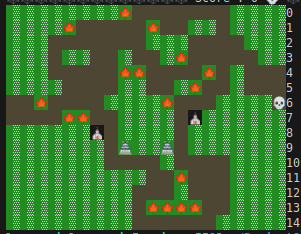
\includegraphics[height = 5cm, width = 9cm]{positionnement.png}
                \caption{Positionnement des tours et des arbres} 
                \label{fig: positionnement } 
            \end{figure}
            \newpage
        \subsection{Dynamique des acteurs}
            Le jeu exhibe une dynamique particulière de mouvement et d'habileté impliquant les protagonistes. Un être monstrueux se meut en suivant un modèle spécifique de déplacement, propre à sa nature, dans le but d'atteindre la sortie du monde, tandis que les tours font face à ces attaques en opposant des contre-offensives.
            \subsubsection{Déplacement simple}
            Un déplacement simple est un mouvement vers une position voisine libre, et c'est le type que les monstres simples suivent. Étant donné que les positions d'entrée et de sortie sont prédéterminées, la stratégie inhérente à ce mode de déplacement consiste à essayer de se déplacer directement en direction de la sortie. En cas d'impossibilité, les acteurs optent alors de manière aléatoire pour une autre position adjacente non occupée. Cette notion de non-déterminisme est introduite afin d'éviter que les acteurs ne soient bloqués en effectuant des allers-retours infinis entre deux positions.
            \subsubsection{Déplacement optimal}\label{optimal chemin}
           
            Le déplacement optimal pour les monstres de type $BigMonster$ implique de suivre le chemin le plus court reliant les positions de départ et d'arrivée dans la grille, tracé à l'aide de l'algorithme de recherche de chemin $A^{*}$. La figure~\ref{fig: Astar_Road } illustre un exemple de chemin entre les positions $(7,0)$ et $(6,19)$ 
            généré par cet algorithme. Il est important de noter que les grands monstres ne peuvent se déplacer que le long de ce chemin et ne peuvent jamais s'en écarter au cours du jeu.
            % \newpage
             \begin{figure}[h]
                \centering
                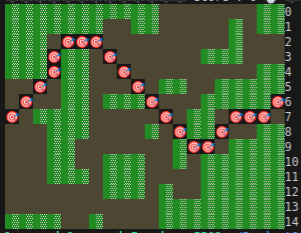
\includegraphics[height = 6cm, width = 10cm]{Astar_Road.png}
                \caption{Chemin optimal} 
                \label{fig: Astar_Road } 
            \end{figure}            
            \subsubsection{Attaque des tours}
                Les tours ont une portée d'attaque connue. Pour les tours simples, elles peuvent infliger des dégâts dans un carré de 5x5 centré sur leur position. L'exemple de cette portée est présenté dans la figure~\ref{fig: SimpleTower}. En revanche, les tours magiques ont une portée plus grande, pouvant attaquer à une distance de trois unités de surface dans les huit directions, comme illustré dans la figure~\ref{fig: MagicTower }.
                  \begin{figure}[h]
                \begin{minipage}[c]{.46\linewidth}
                    \centering
                    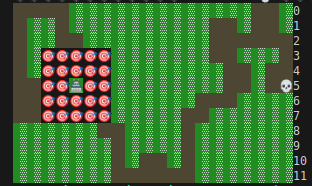
\includegraphics[height=4cm, width = 7cm]{SimpleTowerAttackRange.png}
                    \caption{Une tour simple}
                    \label{fig: SimpleTower}
                \end{minipage}
                \hfill%
                \begin{minipage}[c]{.46\linewidth}
                      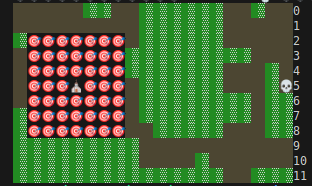
\includegraphics[height=4cm, width = 7cm]{MagicTowerAttackRange.png}
                        \caption{Une tour magique} 
                        \label{fig: MagicTower } 
                \end{minipage}
            \end{figure}
        \subsection{Phases du jeu}\label{phases du jeu}
            Le jeu est organisé en phases : à chaque tour, tous les acteurs du monde peuvent soit se déplacer d'une case voisine, soit rester immobiles, et les tours peuvent effectuer des attaques. De plus, de nouveaux monstres peuvent être introduits dans le jeu. 
            
            La première étape consiste à vérifier s'il est nécessaire d'introduire de nouveaux monstres. Pour les déplacements, un simple monstre peut se déplacer librement vers une case voisine, tandis qu'un grand monstre qui suit un chemin optimal ne peut se déplacer vers une position voisine que si cela le rapproche de sa destination. Sinon, il reste immobile. Les tours effectuent leurs attaques et dès qu'un monstre n'a plus de points de vie, il est éliminé de la grille.
        \subsection{Moteur du jeu}
            Les mouvements des acteurs pendant les phases de jeu sont gérés par le moteur du jeu, qui est l'entité responsable de l'application des mouvements et de la mise à jour des positions dans le monde. Le moteur de jeu reçoit une phase de jeu et filtre les éventuels conflits qui peuvent survenir si deux acteurs tentent d'aller à la même nouvelle position. Dans ce cas, les déplacements des grands monstres sont privilégiés. 
            
            Il est important de noter que le moteur de jeu ne s'occupe que des mouvements des acteurs. Les attaques des tours sont gérées par elles-mêmes, comme expliqué dans la section précédente \ref{phases du jeu}.
        % \subsection{Contrôle du flux des acteurs}
        \subsection{Fin d'une partie}
        Le but du jeu consiste à protéger la position finale contre les ennemis. À chaque tour, on vérifie à l'aide de la fonction $gameOver$ si un monstre a atteint la position finale. Si c'est le cas, le jeu prend fin et les ennemis sont déclarés gagnants, comme le montre l'exemple de la figure~\ref{fig:fin d'une partie}. Dans le cas contraire, la partie se termine si le nombre de tours prévus est écoulé. 
        
        La complexité de la fonction $gameOver$ est en $O(N)$, où $N$ est le nombre d'acteurs dans le monde.
    \begin{figure}[h]
        \centering
        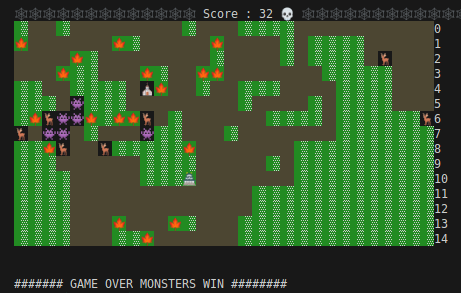
\includegraphics[height = 7cm, width = 12cm ]{Capture d’écran du 2023-05-12 14-11-17.png}
        \caption{Fin d'une partie}
        \label{fig:fin d'une partie}
    \end{figure}
        \newpage
        \subsection{Boucle du jeu}
    
        Une fois que le monde a été créé, on a tracé un chemin aléatoire entre la position de départ et la position finale en utilisant la fonction "Road". Ensuite, on a placé les tours et les arbres dans le monde en utilisant les fonctions "TowersPlacement" et "TreesPlacement". Pour gérer le flux d'ennemis, on a utilisé la fonction "addActorsToWorld" en veillant à ce que la période entre l'entrée de deux ennemis de même type soit égale à 6. Les attaques des tours ont été gérées à l'aide de la fonction "TowersAttacks" pour réduire les points de vie des monstres et les éliminer. 
        
        On a également inclus la fonction "gameOver" pour tester si un ennemi est arrivé à la position finale, sinon la fonction "gamePhase" est utilisée pour déterminer les mouvements de tous les acteurs. Ces mouvements ont ensuite appliqués à l'aide de la fonction "gameMotor". 
        
        La figure ~\ref{fig: game_loop } illustre la représentation de la boucle principale du projet.
    \begin{figure}[h]
                \centering
                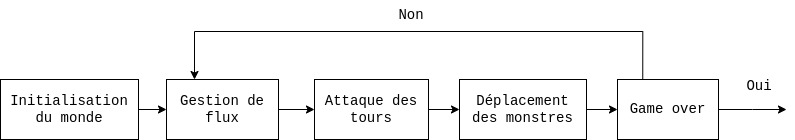
\includegraphics[height = 3.5cm, width = 16cm]{Diagramme sans nom (1).jpg}
                \caption{La boucle principale du jeu} 
                \label{fig: game_loop } 
            \end{figure}
        \subsection{Affichage du jeu} 
    Pour visualiser correctement l’exécution de notre programme, on a eu l’idée d’implémenter un visualiseur en mode terminal qui affiche le monde et les différents acteurs à chaque itération en utilisant les codes d'échappement de couleur, En effet, une fonction display dans le fichier \textit{world.ts}, la figure~\ref{fig: display } représente une visualisation du monde \\
     \begin{figure}[h]
                \centering
                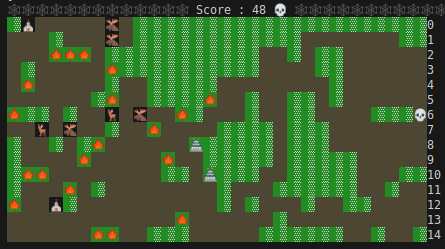
\includegraphics[height = 6cm, width = 10cm]{WorldFigure.png}
                \caption{l'affichage terminal du monde} 
                \label{fig: display } 
            \end{figure}
    % \newpage
    \section{Algorithme A*}
        L'objectif des monstres dans le jeu c'est d'arriver à la position de sortie de la grille, ainsi il convient de trouver une méthode de lier la position initiale avec cette position. En effet, cela introduit une difficulté supplémentaire dans le jeu. Pour cela, on a choisit d'utiliser l'algorithme de recherche de chemin minimal $A^{*}$.
        \subsection{Implémentation}
            L'implémentation adoptée pour cet algorithme utilise les matrices d'adjacence. Elle recourt à une fonction heuristique pour évaluer le coût estimé du chemin le plus court vers la destination, et à une file de priorité pour explorer les sommets du graphe en vue de trouver le chemin optimal. Dans un souci de minimiser les dépendances entre fichiers, une heuristique a été mise en place qui associe la valeur 2 à la première moitié des sommets et la valeur 1 aux autres. Bien que la distance euclidienne eût été envisagée comme heuristique, elle requérait l'emploi de fonctions auxiliaires pour calculer les distances, engendrant une dépendance avec d'autres fichiers et complexifiant l'algorithme.
        \subsection{Adaptation au jeu}
            L'adaptation de l'algorithme au jeu constitue un défi important. Pour optimiser la performance de l'algorithme, seules les positions de la grille appartenant au type "Road" sont considérées comme des sommets du graphe. Les positions de type "Floor" sont donc exclues, car elles sont en grand nombre et ne servent pas dans le déplacement des acteurs. Ensuite, les relations entre ces sommets sont établies dans l'ordre où les positions sont collectées lors du parcours, et la grille est ainsi convertie en graphe. Une fois que l'algorithme $A^{*}$ est appliqué, la fonction récursive \textit{ConstructRoad} est utilisée pour convertir le tableau $parents$, représentant l'arborescence des sommets visités, en un tableau contenant le chemin le plus court reliant la position de départ à la position de sortie de la grille.
        \subsection{Complexité}
            
        La complexité de la fonction $Astar$ est déterminée par la complexité des fonctions appelées en son sein, qui sont $Initialization$, $CalculateDplusHmin$, $GetOutgoingArcs$ et $Relax$.
        La complexité de $Initialization$ est O(N) où N est la taille du graphe G. La complexité de $GetOutgoingArcs$ est O(N) également, car elle parcourt tous les sommets pour trouver les arcs sortants de x. Puis, la complexité de $Heuristic$ est considérée comme constante ici, car la fonction n'estime pas le coût de la solution, elle renvoie simplement une valeur fixe en fonction du sommet. La complexité de $CalculateDplusHmin$ est O(N) également, car elle parcourt tous les sommets gris pour trouver celui ayant la plus petite distance à partir de s.
        
        Enfin, la complexité de Relax est O(1), car elle effectue une mise à jour de la distance et du parent pour chaque arc sortant de x. Au total, la complexité de $Astar$ est donc O(N²) dans le pire des cas, car $CalculateDplusHmin$ est appelé pour chaque sommet gris, et chaque appel parcourt tous les sommets gris pour trouver celui qui minimise d + h.
    \section{Tests}
        \subsection{Tests structurels}
Dans notre projet, nous avons utilisé ESLint pour détecter les erreurs de syntaxe, de style et de logique dans notre code TypeScript, tandis que le framework de test Jest a été utilisé pour écrire et exécuter des tests unitaires.
        \subsubsection{Utilisation de $Jest$}
                $Jest$ est un outil de test unitaire pour TypeScript qui permet de tester des fonctions et des modules individuellement, en s'assurant que chacun d'entre eux fonctionne correctement. Jest utilise une syntaxe claire pour écrire des tests, avec des fonctions telles que "describe", "it" et "expect" qui facilitent la compréhension et la lecture des tests, c'est pour ça qu'on a trouvé que l'utilisation de $jest$ était plus agréable que les "assert" et gcov en C.
        \subsection{Tests fonctionnels}
    Dans notre projet, nous avons effectué plusieurs tests fonctionnels pour nous assurer que les fonctions répondait aux spécifications requises. Parmi les tests que nous avons effectués : 
      \begin{itemize}
    \item Test d'initialisation du monde. Nous initialisons le monde avec différentes conditions et vérifions s'il est dans la position souhaitée 
    \item  Tests des fonctions d'ajout des monstres et des tours dans la matrice.
Ces tests consistent à voir si la position d'ajout d'acteur est bien valable.
    \item Les tests de "gameMotor" et "gameOver" sont parmis les tests fonctionnels du jeu. 
\end{itemize}


    \section{Aspects fonctionnels}
    La programmation fonctionnelle est un paradigme de programmation qui se concentre sur la pureté, la modularité et la citoyenneté de première classe des fonctions.
        \subsection{Pureté}
        Le but de la programmation fonctionnelle consiste à écrire du code pur, c'est-à-dire des fonctions sans effets de bord, afin de simplifier les tests et de rendre les différentes parties du code indépendantes les unes des autres. Pour notre projet, nous avons fait de notre mieux pour minimiser les effets secondaires en créant des fonctions pures telles que \textit{(CreateEmptyMatrix, CreateWorld, getRandomInt, compareActions, getNeighbors, randomPath)}, qui utilisent des constantes et des fonctions d'ordre supérieur \textit{(map, forEach)}. Nous avons également créé des fonctions qui utilisent la récursivité terminale, comme \textit{gameOver}, afin d'éviter les dépassements de pile d'appels.
        \subsection{Modularité}
       Afin de faciliter la compréhension du code et de réduire les dépendances entre les différents fichiers, nous avons adopté une approche de division des tâches. Pour ce faire, nous avons créé des fichiers spécialisés pour chaque fonction, tels que defineType.ts pour stocker les types de données que nous avons construits \textit{actor, point, position, world, move, action} et la liste \textit{ActorsTypeList}, actors.ts pour les fonctions en relation avec les acteurs, \textit{rand\_road.ts} pour les fonctions qui génèrent des chemins aléatoires entre deux points, \textit{movements.ts} pour les mouvements des acteurs, \textit{world.ts} pour la création et l'affichage du monde, \textit{Astar.ts} pour l'algorithme de chemin minimal suivi par les gros monstres, et \textit{game\_loop.ts} pour la boucle principale du jeu. Cette approche a permis de rendre le code plus lisible et de faciliter la compréhension de chaque fonctionnalité.
        \subsection{Citoyenneté de première classe}
        La notion de citoyenneté de première classe est un élément central de la programmation fonctionnelle. Dans notre projet, nous avons mis en pratique cette notion en utilisant la caractéristique de nommage dans la liste \textit{ActorsTypeList} qui contient tous les acteurs implémentés. Chaque acteur est caractérisé par plusieurs champs, notamment un champ \textit{move} pour la fonction qui déplace l'acteur. En considérant les fonctions comme des entités de première classe, nous avons mis en place un système qui nous permet de mieux structurer notre code et de faciliter la manipulation des différents acteurs.
    \section{Améliorations possibles}
    
        \subsection{Optimisation de A*}
        Une autre piste d'améliorations qu'on pourrait faire c'est d'utiliser une implémentation de A* avec la structure de données des tas min. Un tas min est une structure de données de file de priorité implémentée à l'aide d'un arbre binaire complet où le nœud parent est toujours de moindre priorité que ses enfants. En utilisant un tas min, les nœuds sont triés par ordre de priorité, et la file de priorité peut être mise à jour de manière efficace lorsqu'un nœud est ajouté ou retiré.
        
        Le processus de sélection du nœud favori dans chaque itération de l'algorithme A* avec cette méthode est rapide et ne prend pas d'heures supplémentaires. Toutefois, les opérations d'ajout et de suppression de nœuds de la file de priorité ont une complexité de $O(log(n))$, où n est le nombre de nœuds dans le graphe. Il est également possible d'utiliser toutes les positions dans le monde comme nœuds du graphe, ce qui permet de facilement identifier les voisins d'un nœud en utilisant ses vrais voisins dans le monde plutôt que les indices des nœuds dans l'ordre dans lequel elles sont récupérées du monde.
        \subsection{Création d'une page en HTML}
       
        Il est envisageable d'améliorer ce projet en créant une page Web en langage HTML qui permettrait d'afficher le jeu de manière continue. Cela impliquerait d'incorporer des effets visuels entre les différentes phases du jeu, ce qui aurait pour avantage de faciliter la visualisation des changements intervenus au cours de la partie. En outre, cette approche pourrait s'avérer très utile pour établir une communication efficace avec l'utilisateur, notamment pour l'informer des interventions possibles telles que l'ajout de tours. Ceci aura pour effet de renforcer l'engagement de l'utilisateur dans le jeu et de le divertir davantage.
        
        Initialement, nous avions envisagé de convertir le jeu en une page HTML dès le début du projet, mais nous avons rapidement constaté que cette tâche n'était pas aussi simple que nous l'avions imaginée, même avec l'utilisation de $Parcel$. Cependant, nous sommes convaincus que si nous parvenons à surmonter les difficultés techniques rencontrées, cette option sera très bénéfique pour notre projet.
    \section{Conclusion}

   Dans le cadre du "Projet de programmation fonctionnelle", notre équipe s'est engagée dans le développement d'un jeu "Tower Defense". Ce projet nous a permis d'approfondir nos connaissances en programmation fonctionnelle avec TypeScript, ainsi que d'utiliser des outils tels que \textbf{Eslint} et \textbf{Jest} pour faciliter le processus de développement et des tests. Travailler en équipe nous a enseigné l'importance de l'organisation et de la collaboration, et nous avons réalisé l'importance des tests pour assurer la qualité et la fiabilité du code. Dans l'ensemble, cette expérience a été une opportunité unique de maîtriser de nouveaux concepts, d'améliorer nos compétences en programmation et de renforcer notre esprit d'équipe, contribuant ainsi à notre développement professionnel et à notre passion pour la programmation.
   
\end{document}